\begin{figure}[H]
\centering
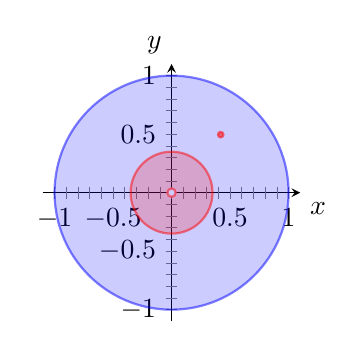
\begin{tikzpicture}
\begin{axis}[%
    width= \linewidth*2/5,
    height= \linewidth*2/5,
    enlargelimits=0,
  axis x line=center,
  axis y line=center,
  xtick={-1,-0.5,...,1},
  ytick={-1,-0.5,...,1},
  xlabel={$x$},
  ylabel={$y$},
  extra x ticks={-0.9,-0.8,...,0.9},
  extra y ticks={-0.9,-0.8,...,0.9},
  extra x tick label={\empty},
  extra y tick label={\empty},
  xlabel style={below right},
  ylabel style={above left},
  xmin=-1.1,
  xmax=1.1,
  ymin=-1.1,
  ymax=1.1]
  \definecolor{auxblue}{rgb}{0.8,0.8,1}
  \draw [fill opacity=0.2, draw opacity=0.5, thick, fill=blue, draw=blue] (0,0) circle (1);
  \draw [fill opacity=0.2, draw opacity=0.5, thick, fill=red, draw=red] (0,0) circle (0.35);
  \draw [fill opacity=0.5, draw opacity=0.5, thick, fill=red, draw=red] (0.42,0.49608467019) circle (1pt);
  \draw [thick, draw opacity=0.5, fill=auxblue, draw=red] (0,0) circle (1.5pt);
  
\end{axis}
\end{tikzpicture}
\caption{$B_1 \left( 0,0 \right)$ y $B_1 \left( \frac{42}{100},\sqrt{\frac{2461}{10}} \right)$}
\end{figure}
